\section{相对论重离子对撞}

正如 \ref{夸克胶子等离子体} 一节中所提到的一样,在实验上产生夸克胶子等离子体的主要方式为相对论重离子对撞。通过控制相对论重离子对撞的离子类型和对撞中每核子对的能量($\sqrt{s_{NN}}$),可以在QCD的相图中得到不同的T-$\mu_b$曲线。从而成为探索QCD相图的有力的工具。以相对论重离子对撞机(Relativistic Heavy-Ion Collider, RHIC)为例。常用的对撞系统为金-金对撞,最高可以达到 \sNNerbai 的对撞能量,在这种情况下金离子可以被加速到大约99.99\%的光速。

在相对论情况下球状的原子核会收缩成扁平的盘状,当他们在束流管中交汇时就可能发生对撞。一个很重要的描述对撞对心程度的参数为碰撞参数b,其定义为两个核中心之间的距离,参见图 \ref{fig:ImpactParameter}。当$b \approx 0$时称为“中心(Central)”对撞,当$b \approx 2R$时称为“偏心(Peripheral)”对撞。但在实验上我们无法直接观测到一次对撞发生时的碰撞参数,所以我们用一个基于带电粒子多重数(在某区间内的带电粒子数,Reference Multiplicity,RefMult)的中心度(Centrality)定义来描述对撞的对心程度。Glauber模型被用来计算对撞发生后带电粒子多重数的分布,在Glauber模型中带电粒子多重数和中心度关系的示意图见图 \ref{fig:Centrality}。除了中心度,还有一些常用的量也被用来描述对撞的对心程度,例如参加对撞核子数($N_{part}$),二元碰撞数($N_{bin}$)以及核几何重叠函数(Geometrical nuclear overlap function, $T_{AA} = N_{coll}/\sigma_{NN}^{inel}$)等。

\begin{figure}[htb]
    \begin{center}
    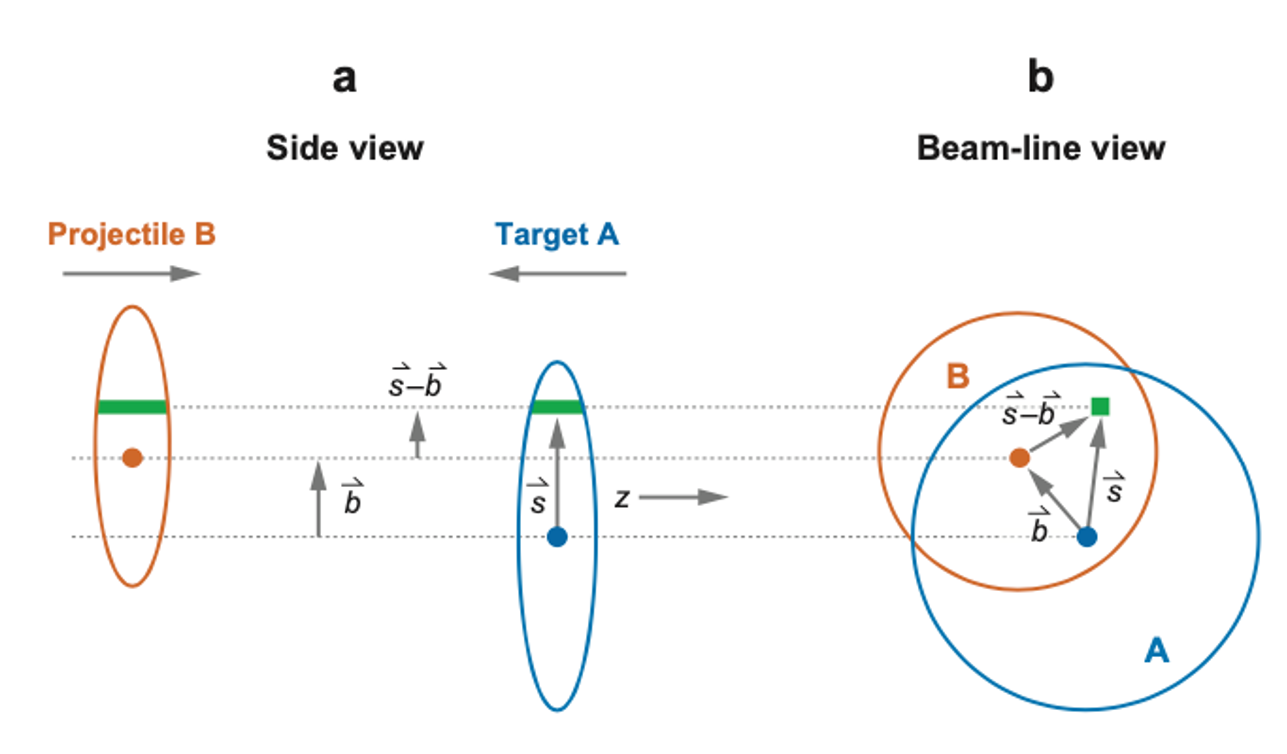
\includegraphics[width=0.7\textwidth,clip]{figures/Chapter1/ImpactParameter.png}
    \end{center}
    \caption[重离子对撞中的碰撞参数示意图]{重离子对撞中的碰撞参数示意图,其中图(a)为侧视图,图(b)为沿着束流方向视图。$\overrightarrow{b}$为碰撞参数,$\overrightarrow{s}$为Glauber模型中表示到核子中心距离的向量}
    \label{fig:ImpactParameter}
\end{figure}

\begin{figure}[htb]
    \begin{center}
    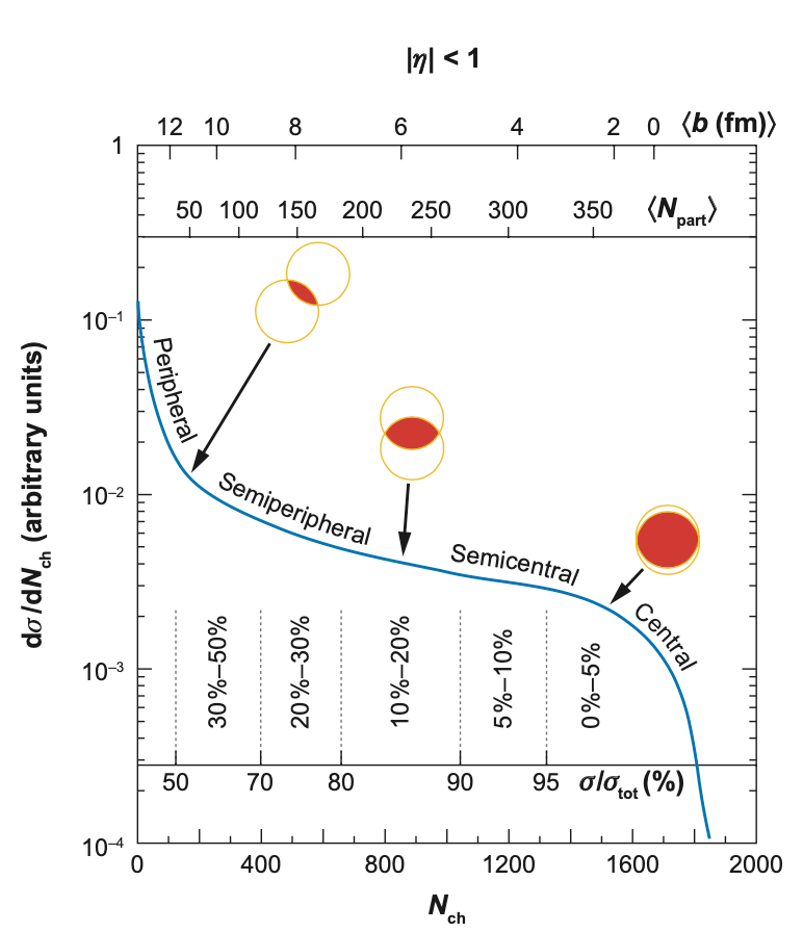
\includegraphics[width=0.6\textwidth,clip]{figures/Chapter1/Centrality.png}
    \end{center}
    \caption[中心度定义示意图]{Glauber模型中末态可观测的带电粒子径迹数和碰撞参数以及$N_{part}$的关系示意图,图中的值为定性的分布,并不是实际的测量值}
    \label{fig:Centrality}
\end{figure}

在一次重离子对撞发生以后所产生的物质如何演化是重离子对撞物理中最为感兴趣的问题。对撞发生后的系统演化的示意图见图 \ref{fig:HIC}。在碰撞的早期发生的过程主要是核子和核子之间(或者说核子内的部分子)之间的散射过程,主要是有着小横动量转移的“软(soft)”过程。在这个阶段,虽然数量较少但仍有一部分粒子发生了大横动量转移的过程(“硬(hard)”过程),产生了有着较高横动量($p_T$)的粒子,这些硬过程对我们的研究十分重要。碰撞发生的早期阶段被称作“预平衡”阶段,目前有多种理论模型来描述这个阶段,例如色玻璃凝聚模型(Color Glass Condensate, CGC),但总的来说对他们的动力学状态仍不是十分清楚。在碰撞发生后的大约 1 fm/c 之后,发生对撞的两个离子相互离开,但是在离子和离子重叠的区域沉积下了大量的能量,在这个时间段能量密度可以达到大约 $12 {\rm~GeV/fm^{-3}}$,远大于强子内的能量密度,因此对撞中产生的夸克和胶子等难以保持束缚的强子态,组成一种新的物质的态,正是之前提到的夸克胶子等离子体。近些年来一些粘性流体力学的模型被用来描述夸克胶子等离子体的性质并且取得了巨大的成功。

在之后,夸克胶子等离子体向各个方向扩张同时冷却,当系统的温度接近$T_c \approx 150 {\rm~MeV}$的时候系统开始冷却,首先夸克和胶子强子化生成各种强子,从夸克胶子等离子体相向强子气相转变,在这个过程中强子和强子之间仍可以发生非弹性散射,粒子的种类仍会发生改变产生新的粒子。当强子的产额基本固定之后称这个状态为化学冻结(Chemical freeze-out)。 之后随着温度的进一步降低和系统的扩张,当粒子之间的距离大于粒子散射的平均自由程时,粒子的动力学性质也几乎不再改变,这个状态被称为动力学冻结(Kinetic freeze-out)。动力学冻结发生后粒子的动量谱便不再改变并且自由地向各个方向飞出并被探测器探测到。

可以看到,整个夸克胶子等离子体的演化时间极短,远小于现今的探测器可以做到的最小的时间分辨,这意味着我们需要从探测到的末态粒子来反推夸克胶子等离子体的性质和初始状态,这就要求找到一些合适的物理探针来进行夸克胶子等离子体的研究。从图 \ref{fig:HIC} 中可以看到,光子和电子可以在夸克胶子等离子体演化的整个过程中产生,又因为其又几乎不与强子物质发生反应,可以在末态被探测到并且受到较小的介质影响。是一个研究夸克胶子等离子体的理想探针,将会在下一节中进行详细的介绍。

% \begin{figure}[htb]
%     \begin{center}
%     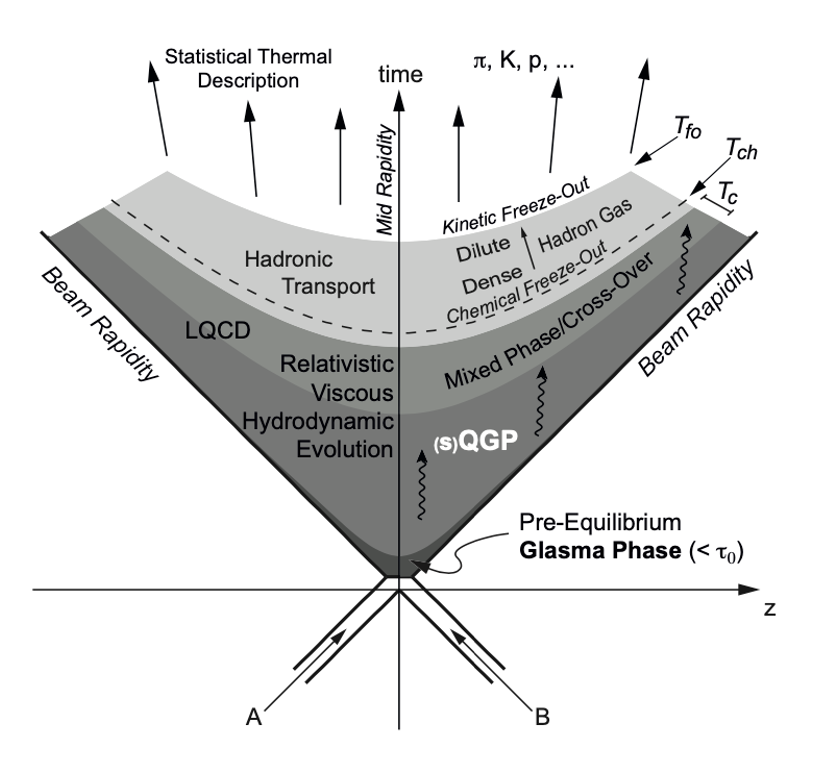
\includegraphics[width=0.8\textwidth,clip]{figures/Chapter1/HIC.png}
%     \end{center}
%     \caption[重离子对撞演化示意图]{一次重离子对撞发生后的系统演化的光锥示意图。主要的相和演化步骤以及对应的温度在图的右侧标出,成功的描述这种演化的模型在图的左侧被标出}
%     \label{fig:HIC}
% \end{figure}

\begin{figure}[htb]
    \begin{center}
    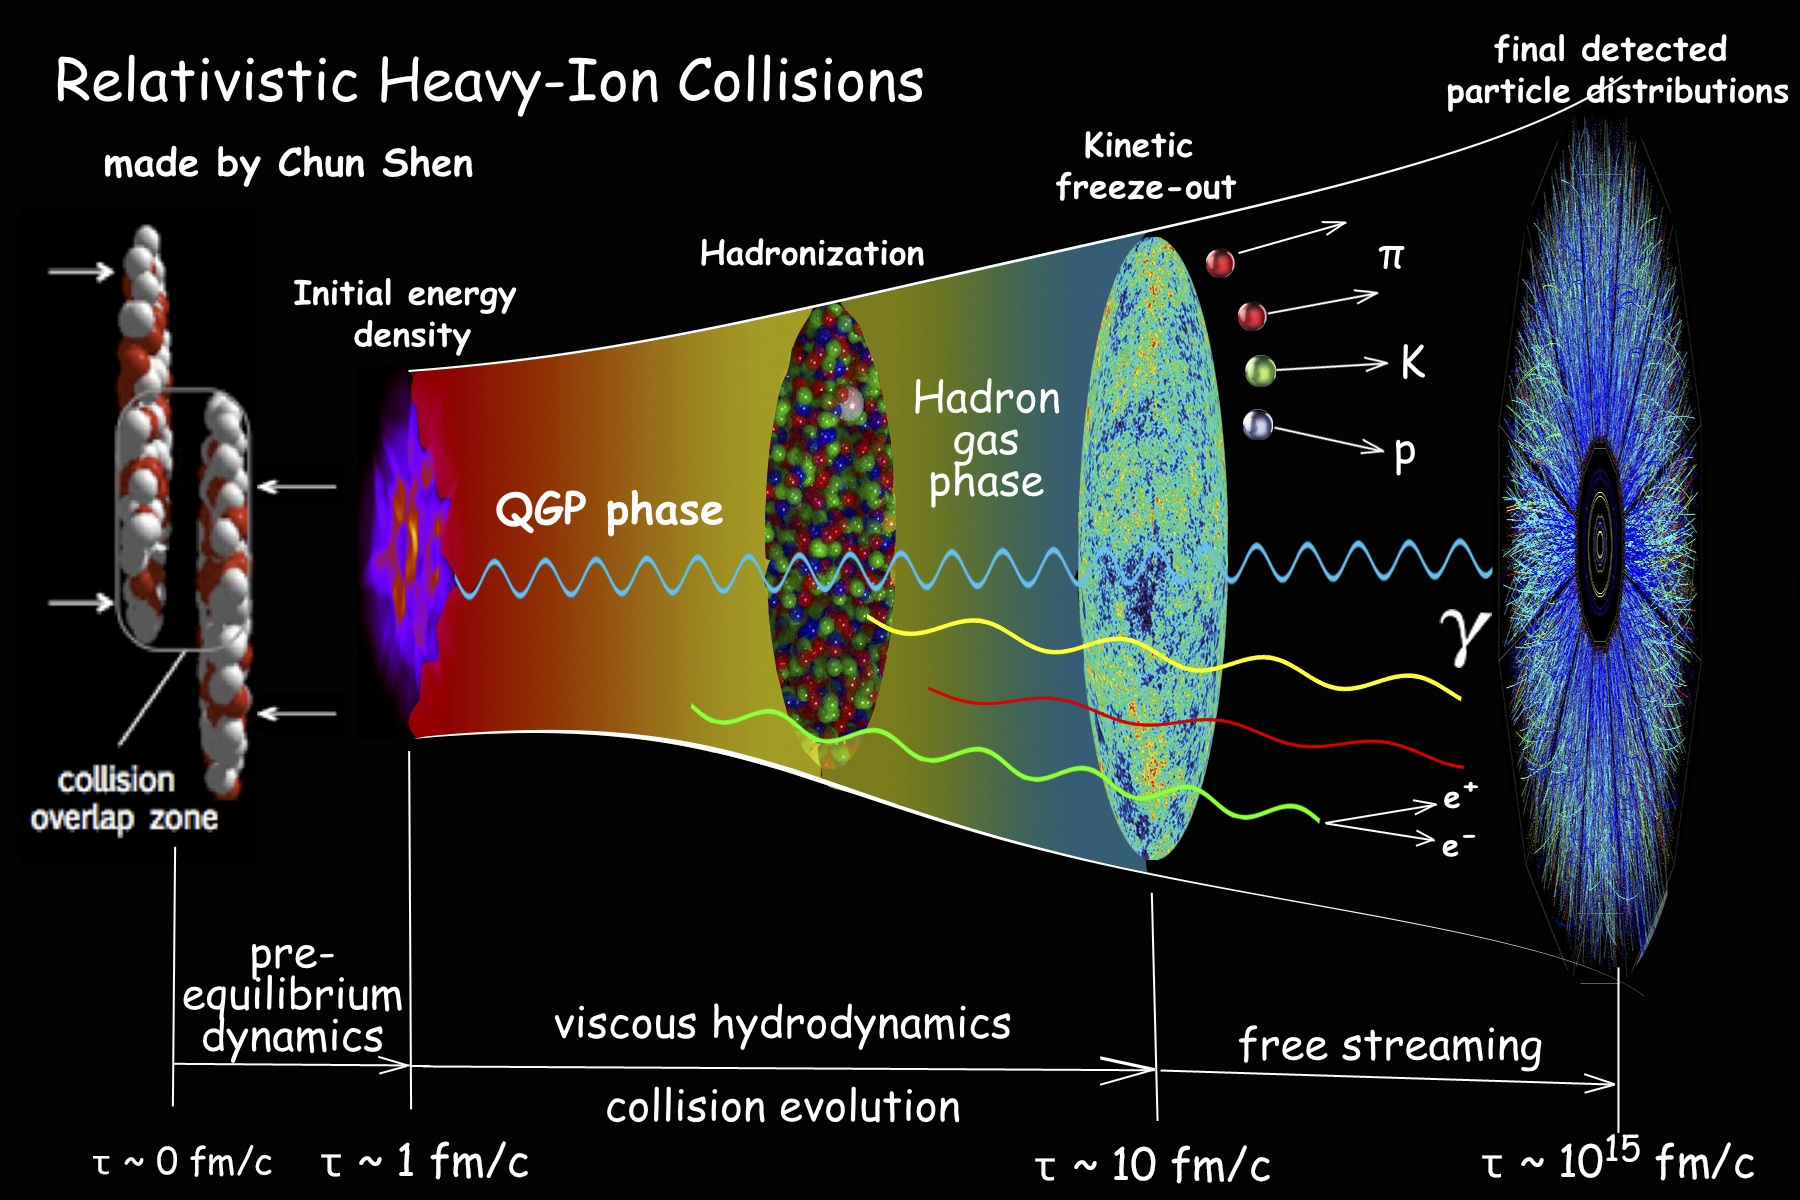
\includegraphics[width=0.8\textwidth,clip]{figures/Chapter1/little_bang-10wt2pd.jpeg}
    \end{center}
    \caption[相对论重离子演化示意图]{一次重离子对撞发生后的系统演化的示意图。图源https://u.osu.edu/vishnu/2014/08/06/sketch-of-relativistic-heavy-ion-collisions/}
    \label{fig:HIC}
\end{figure}